\documentclass[11pt]{article}
\title{Meccano triangles}
\author{https://github.com/heptagons/meccano/nest}
\date{}

\newfam\bbbfam
\font\bbbten=msbm10
\font\bbbseven=msbm7
\font\bbbfive=msbm5
\textfont\bbbfam=\bbbten
\scriptfont\bbbfam=\bbbseven
\scriptscriptfont\bbbfam=\bbbfive
\def\bbb{\fam=\bbbfam}

\usepackage{../../meccano}
\begin{document}

\maketitle
\begin{abstract}
We construct meccano triangles with integers sides and calculate the diagonal distances.
Such diagonals then are used as the new side of more complicated triangles and then again we
calculate new distances formed and so on. Eventually we expect to
find certain angles which can be used to construct regular polygons or something else.
\end{abstract}

\begin{figure}[htp]
\centering
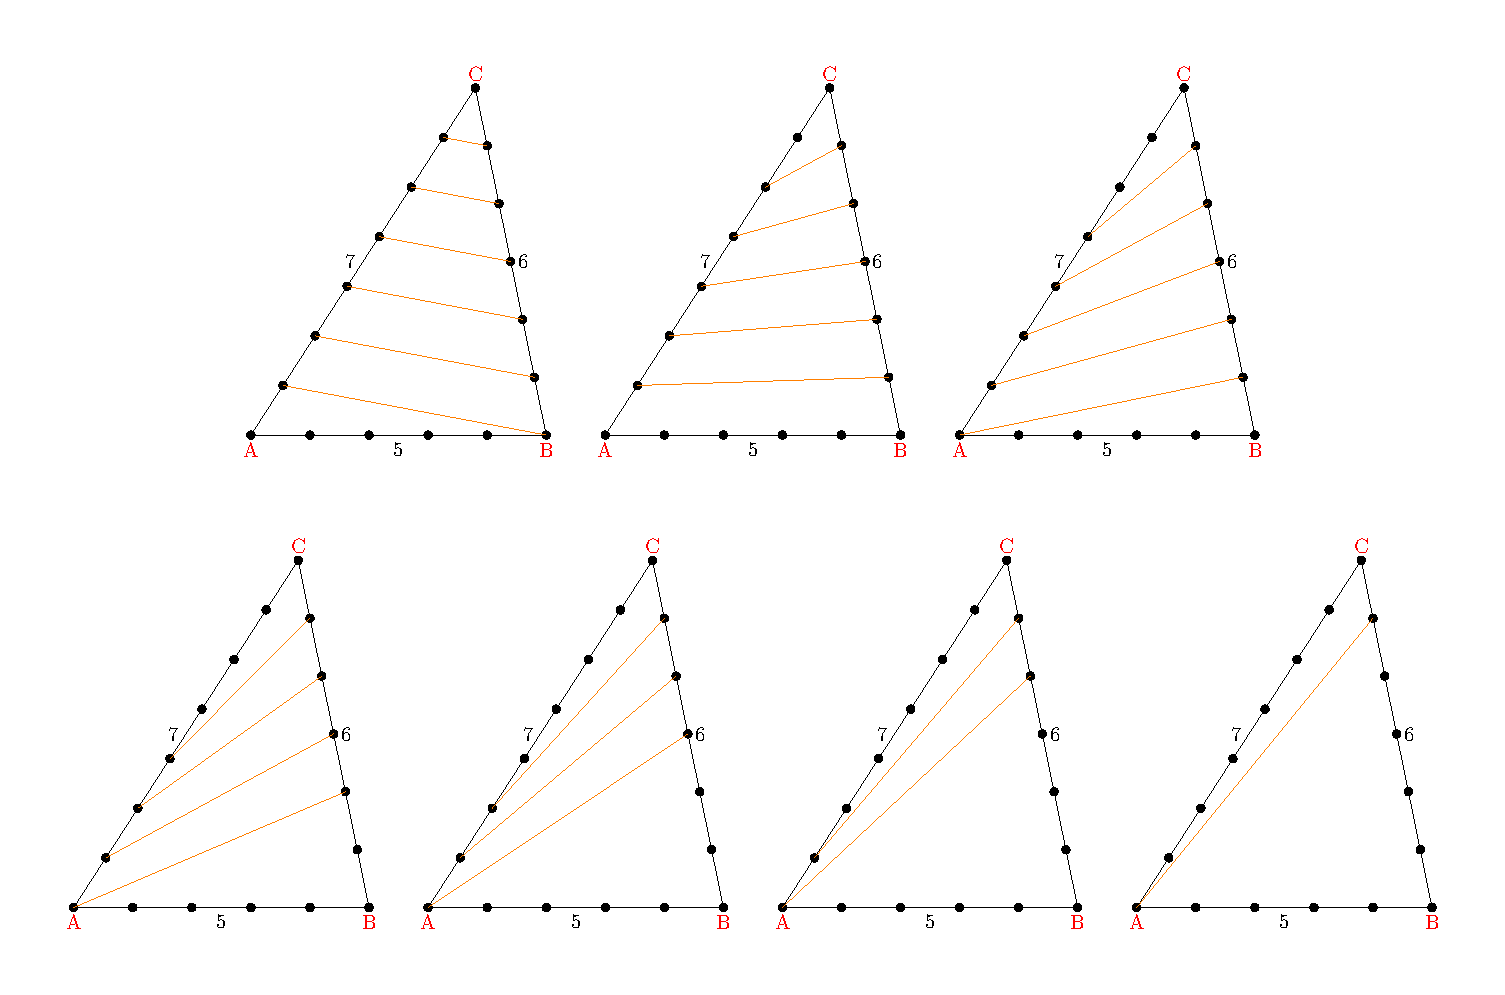
\includegraphics[scale=0.78]{t765}
\caption{The meccano scalene triangle with sides $7$, $6$ and $5$.}
\label{t765}
\end{figure}
\
\section{Meccano triangle}
A meccano triangle has the tree sides $a$, $b$ and $c$ where $a,b,c \in \bbb N$. To avoid repetitions we
consider only the cases $a \ge b$, $b \ge c$ and $a \ge c$. Valid triangles also need the 
condition $a \ge b + c$.

\subsection{Triangle diagonals}
Figure \ref{t765} show a meccano triangle with sides $a=7$, $b=6$ and $c=5$. We have seven groups of diagonals shown as orange lines. The diagonals join points from side $a$ to side $b$ in all combinations. From top to bottom and left to right the groups are:
\begin{center}
\begin{tabular}{||c c c||} 
 \hline
 Group & $a-b$ & diagonals \\ [0.5ex] 
 \hline\hline
 1 & 0 & $a_1b_1$ to $a_6b_6$ \\ 
 \hline
 2 & 1 & $a_2b_1$ to $a_6b_5$ \\
 \hline
 3 & 2 & $a_3b_1$ to $a_7b_5$ \\
 \hline
 4 & 3 & $a_4b_1$ to $a_7b_5$ \\
 \hline
 5 & 4 & $a_5b_1$ to $a_7b_3$ \\
 \hline
 6 & 5 & $a_6b_1$ to $a_7b_2$ \\
 \hline
 7 & 6 & $a_7b1$ \\
 \hline
\end{tabular}
\end{center}

To calculate the diagonals we start calculating $\cos{C}$ where $C$ is the
opposite angle of side $c=5$:
\begin{align}
\cos{C} &= \frac{a^2 + b^2 - c^2}{2ab}\\
        &= \frac{7^2 + 6^2 - 5^2}{2\times7\times6} = \frac{4}{21}
\end{align}

Then with the $\cos{C}$ we can calculate every diagonal $\overline{a_xb_y}$ with:
\begin{align}
\overline{a_xb_y} &= \sqrt{x^2 + y^2 - 2xy\cos{C}}\\
       &= \sqrt{x^2 + y^2 - 2xy\frac{a^2 + b^2 - c^2}{2ab}}
\end{align}

where $1 \le x \le a$, $1 \le y \le b$ and $x - y \ge 0$.

By inspection we deduce that for first meccano triangles:
\begin{align}
a, b, c &\in \bbb{N}\\
\cos{A}, \cos{B}, \cos{C} &\in \bbb{Q}\\
\overline{a_xb_y}, \overline{b_yc_z}, \overline{a_xc_z} &\in \bbb{A}
\end{align}



\end{document}